% =====================================================================
%  Chapter 21 — The Sharpe Ratio and Its Estimation Error
% =====================================================================

\chapter{The Sharpe Ratio and Its Estimation Error}
\label{ch:sharpe}

The Sharpe ratio is the book's summary statistic and the most misused
number in applied finance. This chapter derives its estimation error,
shows why serial correlation makes it worse than the textbook formula
says, and states the correction the book applies.

\section{The definition and the trap in it}

For a strategy with excess returns \(r_1, \dots, r_T\), the Sharpe ratio
is
\begin{equation}
\widehat{SR} = \frac{\bar{r}}{s},
\qquad
\bar{r} = \frac{1}{T}\sum_{t=1}^{T} r_t,
\qquad
s^2 = \frac{1}{T-1}\sum_{t=1}^{T}(r_t - \bar{r})^2.
\end{equation}

The trap is that the textbook standard error,
\begin{equation}
\mathrm{SE}(\widehat{SR}) \approx \frac{1}{\sqrt{T-1}},
\end{equation}
is derived under the assumption that the returns are serially independent.
Monthly strategy returns are not. They have negative autocorrelation from
the no-trade band and from the mean reversion in the tilt; they have
positive autocorrelation from the momentum features and from the
volatility governor, which scales exposure down after a bad period and
therefore produces a run of low returns followed by a run of higher
returns.

\section{Lo's correction}

Lo's 2002 result in the \emph{Financial Analysts Journal} states that the
true sampling variance of the Sharpe ratio is inflated by a scale factor
\(\eta\) that depends on the sample length and on the sum of the
autocorrelations:
\begin{equation}
\eta(q) = \sqrt{q}\left[1 + \frac{2\rho}{1-\rho}
  \left(1 - \frac{1-\rho^{q}}{q(1-\rho)}\right)\right]^{-1/2},
\end{equation}
where \(q\) is the number of observations, \(\rho\) is the sum of the
autocorrelations at lags one and beyond, and the estimate of the Sharpe
ratio is divided by \(\eta(q)\) to give the corrected statistic.

The correction is severe, and the numbers are worth remembering. For
twelve years of monthly data and no autocorrelation, \(\eta\) is about
3.46 --- so the naive standard error understates the true one by more
than a factor of three. With positive autocorrelation of 0.20, \(\eta\)
falls to about 2.07, because positive autocorrelation means the returns
cluster and the effective sample size is smaller than the nominal one.
With negative autocorrelation, \(\eta\) is larger still.

The general lesson is that the naive standard error is wrong in the
optimistic direction for the strategies that most people build. A
strategy with a momentum signal and a volatility governor has positively
correlated returns, and its Sharpe ratio is therefore more uncertain than
the textbook formula suggests.

\begin{figure}[!htbp]
\centering
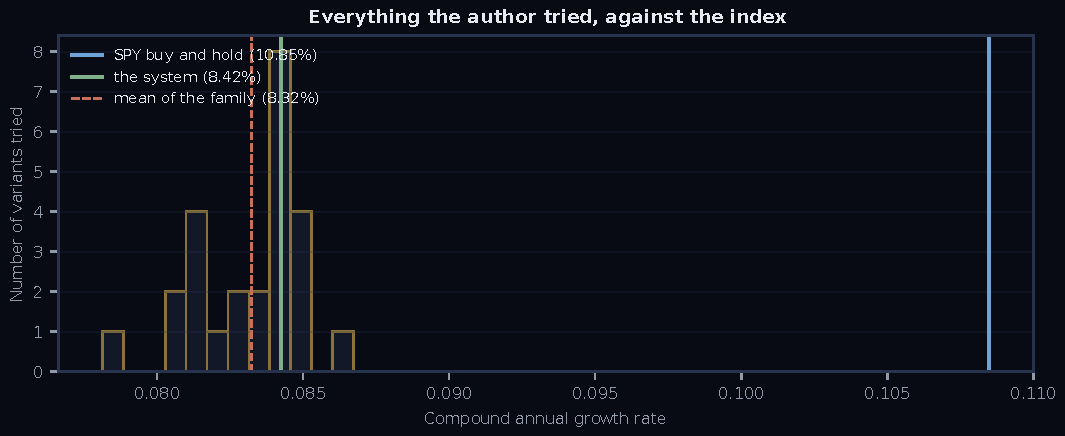
\includegraphics[width=\textwidth]{../figures/fig_family.pdf}
\caption{The trial family. Each member is a complete alternative system
that the book actually ran. The point of the figure is the spread: the
best member's number is the maximum of a noisy sample, and Chapter 22
prices what that maximum is worth.}
\label{fig:family}
\end{figure}

\begin{takeaway}[Lo's correction in one line]
Divide the estimated Sharpe ratio by \(\eta(q)\), where \(\eta\) grows with
the sample length and shrinks with positive autocorrelation. For twelve
years of monthly data with no autocorrelation, \(\eta \approx 3.46\), so
the naive standard error is optimistic by more than a factor of three.
\end{takeaway}

\section{What the book computes}

For every strategy it evaluates --- the system, each member of the trial
family, each comparator, each layer attribution --- the book reports the
naive Sharpe ratio, Lo's scale factor \(\eta\), the first-order
autocorrelation of the returns, and the corrected Sharpe ratio
\(\widehat{SR}/\eta\).

It reports both because they answer different questions. The naive Sharpe
ratio is what the strategy's own record shows, and it is the number a
reader should compare with a benchmark's naive Sharpe ratio computed the
same way. The corrected Sharpe ratio is what is comparable to the
\emph{theoretical} expectation of the maximum Sharpe ratio across a family
of trials, which is what the Deflated Sharpe Ratio of Chapter 22 requires.

The book also reports the Sharpe ratio on the \emph{geometric} return
basis where the comparison demands it, because the difference between the
arithmetic and geometric Sharpe ratios is exactly the \(\sigma^2/2\) term
of Chapter 2, and a strategy's geometric Sharpe ratio is what determines
whether the reader's money compounds.

\section{Why the Sharpe ratio is not the primary statistic anyway}

A final word on the choice of statistic, because the book reports many and
the reader should know which is load-bearing.

The Sharpe ratio is a mean-to-variation ratio and it is the right statistic
for the question ``is this return stream efficient?''. But the owner's
question is ``does this make money and protect principal?'', and for that
question the compound growth rate and the maximum drawdown are more
direct. The Sharpe ratio's role in this book is narrower and more
specific: it is the quantity that the selection machinery operates on,
because the Deflated Sharpe Ratio, the probability of backtest overfitting
and the reality check are all defined in terms of it.

So the book reports a family of statistics, and it says which is which.
The compound growth rate is the money. The maximum drawdown and the time
to recovery are the protection. The Sharpe ratio, in both its naive and
corrected forms, is the thing the selection tests are about.

\begin{keytakeaways}
\item The textbook standard error of the Sharpe ratio assumes independent
returns, and the strategies that most people build have positively
correlated returns, so the textbook error is optimistic for them.
\item Lo's scale factor \(\eta(q)\) is about 3.46 for twelve years of
monthly data with no autocorrelation and about 2.07 with positive
autocorrelation of 0.20.
\item The book reports the naive Sharpe ratio for comparison with a
benchmark computed the same way, and the corrected ratio for comparison
with the theoretical maximum across a trial family.
\item The compound growth rate is the money and the drawdown is the
protection; the Sharpe ratio is load-bearing only as the statistic the
selection machinery operates on.
\end{keytakeaways}
